\subsection{テストレベル}
テストレベルは、何を対象にテストするか、どの目的でテストするかによって分けられる。大きなシステムでは、単体、結合、システム、受入という四つの段階で考えると理解しやすい。ただし、これらは開発プロセスを固定するものではなく、どれが常に最重要というものでもない。

\subsubsection{テスト対象}
\paragraph{単体テスト}
単体テストは、個別にテストできる要素を単独で確認する活動である。対象は、関数、クラス、モジュール、コンポーネント、サブシステムなどである。多くの場合、コードを書いた開発者が実施するが、必ずしもそれに限られない。単体テストの目的は、欠陥を早く見つけ、後段の結合やシステムテストに欠陥を持ち込まないことである。

\paragraph{結合テスト}
結合テストは、複数の要素の相互作用を確認する活動である。モジュール間、コンポーネント間、外部システムとのインタフェース、ハードウェアや運用環境とのやり取りが対象になる。上位から下位へ進めるトップダウン、下位から上位へ進めるボトムアップ、混合方式、一度に結合するビッグバン方式などがある。

\paragraph{システムテスト}
システムテストは、システム全体の振る舞いを確認する活動である。単体テストと結合テストで多くの欠陥は見つかっているはずだが、システム全体で初めて現れる問題もある。機能だけでなく、セキュリティ、プライバシー、速度、正確性、信頼性などの非機能要求の確認にも適している。

\paragraph{受入テスト}
受入テストは、システムが要求とエンドユーザの期待を満たし、利用または配備に進めるかを確認する活動である。利用者や顧客とともに実施されることが多い。運用受入、使いやすさ確認、業務シナリオ確認などを含む。受け入れテスト駆動開発では、機能を実装する前に受入条件を定義する。

\begin{figure}[htbp]
\centering
\IfFileExists{assets/generated_figures/ch05/fig-ch05-04.png}{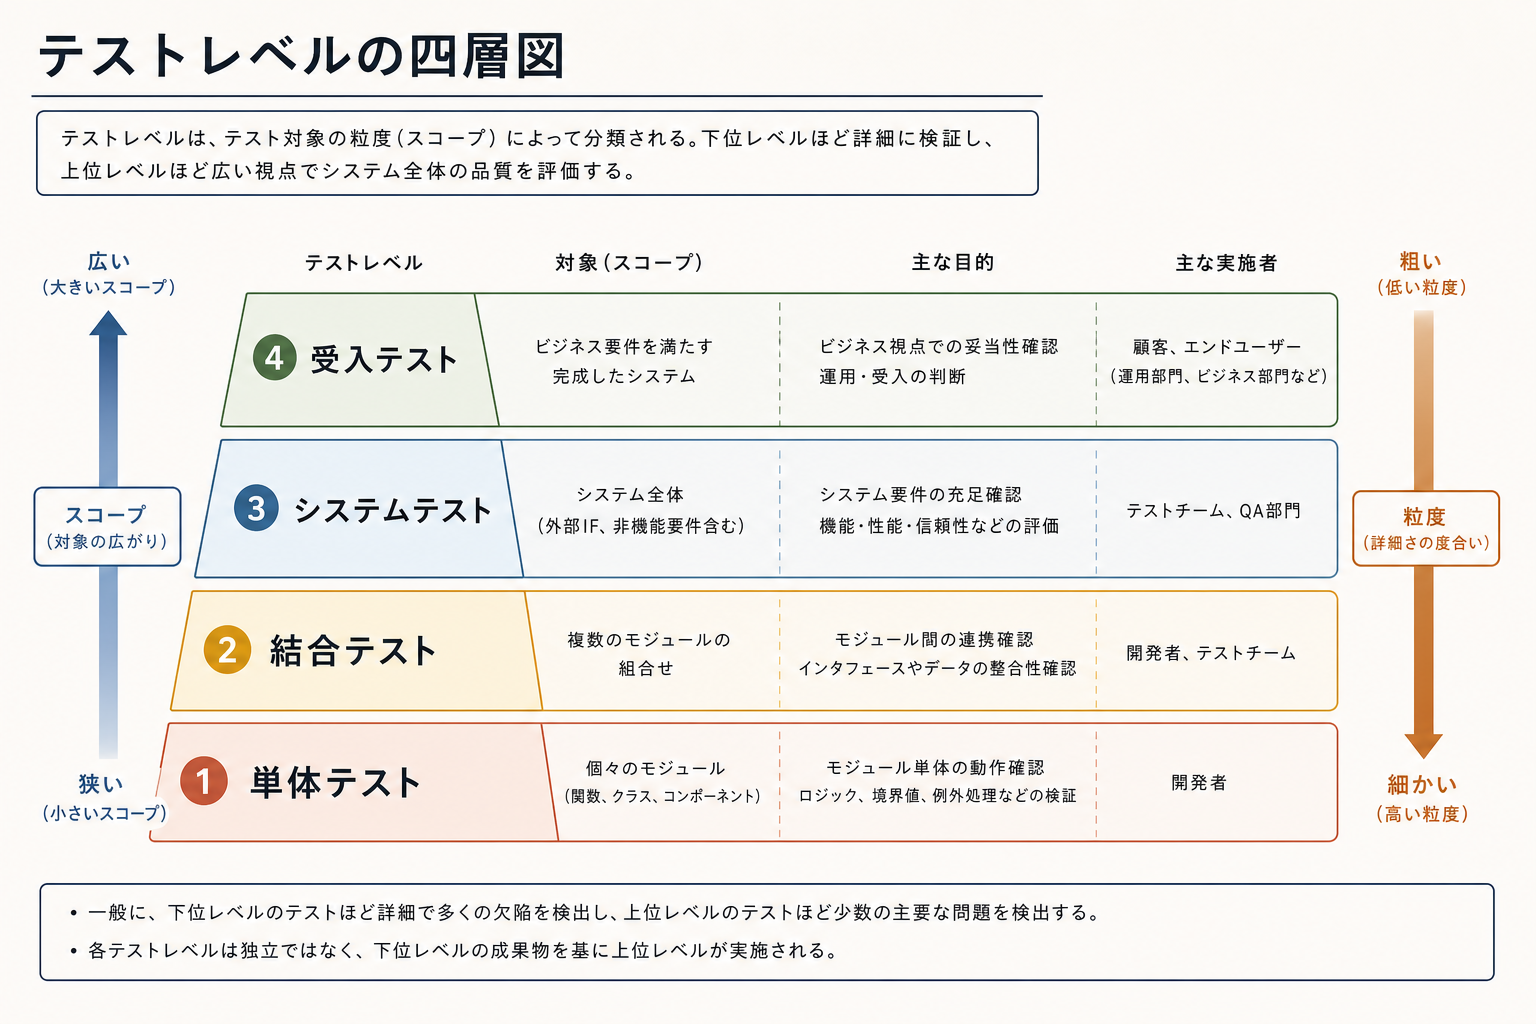
\includegraphics[width=0.96\linewidth]{assets/generated_figures/ch05/fig-ch05-04.png}}{\fbox{\parbox[c][48mm][c]{0.9\linewidth}{\centering 画像生成待ち\\テストレベルの四層図}}}
\caption{テストレベルの四層図}
\label{fig:ch05-04}
\end{figure}

\subsubsection{テスト目的}
テスト目的は、何を確認したいかを表す。目的を明確にすると、テストケースの選び方、測り方、終了判断が決めやすくなる。

\paragraph{適合性テスト}
適合性テストは、SUT が標準、規則、仕様、要求、設計、プロセス、慣行に合っているかを確認する。

\paragraph{法令・規制順守テスト}
法令・規制順守テストは、SUT が法律や規制に従っていることを示す。外部の規制機関や認証制度によって求められることが多い。

\paragraph{導入テスト}
導入テストは、SUT を対象環境へ導入した後に、ハードウェア構成、運用制約、インストール手順を含めて確認する活動である。

\paragraph{アルファテストとベータテスト}
アルファテストは、リリース前に少数の選ばれた利用者に試してもらう活動である。ベータテストは、より広い代表的利用者に試してもらう活動である。いずれも、利用者から問題報告を受けるために行う。

\paragraph{回帰テスト}
回帰テストは、変更後に意図しない悪影響が出ていないことを確認する再テストである。アジャイル、DevOps、テスト駆動開発、継続的開発では特に重要である。すべてのテストを毎回実行するのは高コストなので、選択、最小化、優先順位付けがよく使われる。

\paragraph{優先順位付けテスト}
優先順位付けテストは、テストケースの実行順を工夫し、早い段階で重要な障害を見つけることを狙う。類似していないテストケースから先に実行する類似度ベースの方法などがある。

\paragraph{非機能テスト}
非機能テストは、性能、使いやすさ、信頼性などの非機能面を確認する。代表的な種類を表に示す。

\par\smallskip\noindent\refstepcounter{table}\label{tab:ch05-02}\textbf{表 \thetable: 第05章 ソフトウェアテスト 表02}\par\smallskip
\begin{longtable}{P{0.24\linewidth}P{0.66\linewidth}}
\toprule
\textbf{種類} & \textbf{確認すること} \\
\midrule
性能テスト & 応答時間、処理能力、容量など、性能要求を満たすかを確認する。\\
負荷テスト & 多数の要求や高負荷時に、デッドロック、競合、メモリ漏れ、安定性問題が出ないかを確認する。\\
ストレステスト & 想定を超える負荷を与え、限界や破綻の仕方を確認する。\\
容量テスト & 内部保存容量、データ交換量、情報量に対する限界を確認する。\\
フェイルオーバーテスト & 障害や高負荷時にも、予備資源や代替経路でサービスを継続できるかを確認する。\\
信頼性テスト & 運用プロファイルなどを用いて、将来の信頼性を評価する。\\
互換性テスト & 異なるハードウェア、ソフトウェア、バージョン、リリースと協調できるかを確認する。\\
拡張性テスト & 利用者数、取引数、データ量が増えた場合に対応できるかを確認する。\\
弾力性テスト & クラウドなどで、計算資源、記憶資源、保存資源を増減しても能力を保てるかを確認する。\\
インフラテスト & インフラ構成要素を確認し、停止時間を減らし性能を改善する。\\
バックツーバックテスト & 複数の実装や版に同じ入力を与え、出力差を分析する。\\
回復テスト & クラッシュや災害後に再起動・復旧できるかを確認する。\\
\bottomrule
\end{longtable}

\paragraph{セキュリティテスト}
セキュリティテストは、外部攻撃から SUT とデータを守れるかを確認する。主に機密性、完全性、可用性を扱う。誤用や悪用に対してシステムがどう振る舞うかを確認する負のテストも重要である。

\paragraph{プライバシーテスト}
プライバシーテストは、利用者の個人データを安全に扱い、情報共有方針やプライバシー方針を守れているかを確認する。

\paragraph{インタフェースおよび API テスト}
インタフェーステストは、コンポーネント間でデータや制御情報が正しく交換されるかを確認する。API テストでは、エンドユーザのアプリケーションが API を呼び出す状況を想定し、パラメータ、環境条件、内部データを組み合わせて確認する。

\paragraph{構成テスト}
構成テストは、複数の利用者、環境、設定に対応するソフトウェアが、指定された構成で正しく動くかを確認する。

\paragraph{使いやすさと人間コンピュータ相互作用テスト}
使いやすさテストは、エンドユーザがソフトウェアを学び、使い、誤りから回復できるかを確認する。機能、文書、画面、操作手順、エラー回復が対象になる。

\begin{figure}[htbp]
\centering
\IfFileExists{assets/generated_figures/ch05/fig-ch05-05.png}{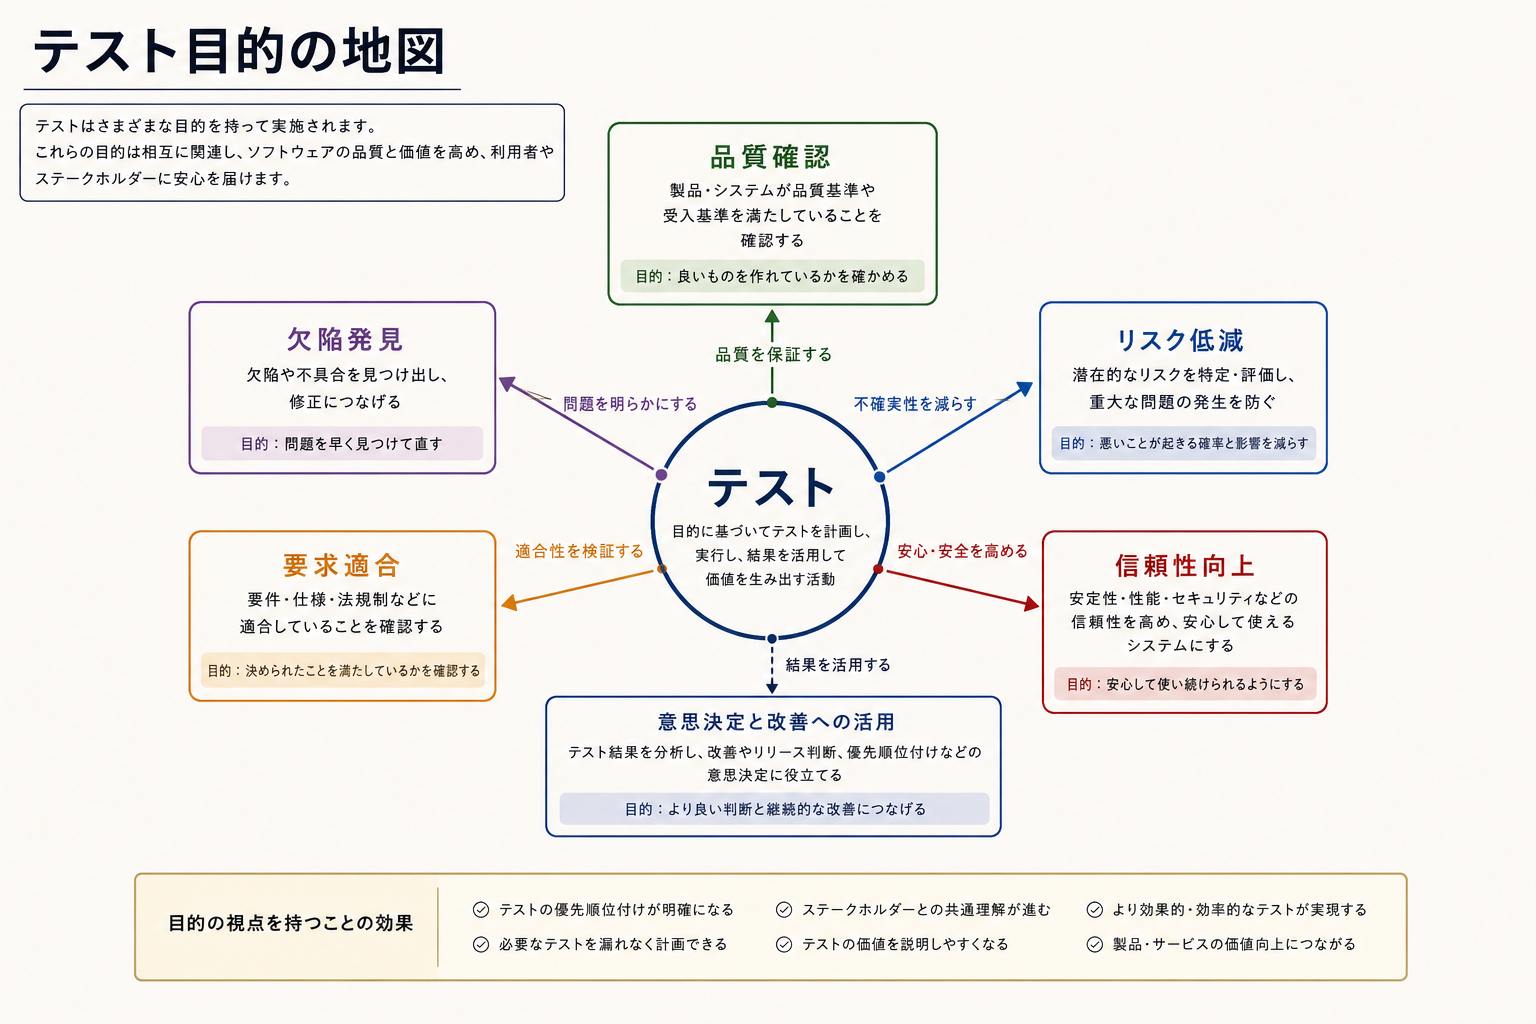
\includegraphics[width=0.96\linewidth]{assets/generated_figures/ch05/fig-ch05-05.png}}{\fbox{\parbox[c][48mm][c]{0.9\linewidth}{\centering 画像生成待ち\\テスト目的の地図}}}
\caption{テスト目的の地図}
\label{fig:ch05-05}
\end{figure}
